% *******************************************************************************
% * Copyright (c) 2007 by Elexis
% * All rights reserved. This document and the accompanying materials
% * are made available under the terms of the Eclipse Public License v1.0
% * which accompanies this distribution, and is available at
% * http://www.eclipse.org/legal/epl-v10.html
% *
% * Contributors:
% *    G. Weirich
% *
% *  $Id: multiuser.tex 4904 2009-01-03 17:58:33Z rgw_ch $
% *******************************************************************************
% !Mode:: "TeX:UTF-8" (encoding info for WinEdt)

\section{Introduction}
\index{Cabinet communautaire}\index{Cabinet de groupe}\index{Centre de santé}
Elexis a d'emblée une conception qui permet l'utilisation par plusieurs utilisateurs et mandants. Il n'y a pas de limitations concernant le nombre d'utilisateurs et mandants. Il n'y a pas non plus des changements à faire lorsqu'on change d'un utilisateur unique à un fonctionnement multi-client.
Dans ce chapitre il y aura juste la présentation de quelques conceptions qui pourraient être utiles dans un fonctionnement multi-utilisateur et multi-mandant.


\section{Rôles (anciennement groupes) et droits}
\label{sec:gruppen}
\index{groupes}\index{rôles}
Dès qu'il y a plusieurs utilisateurs qui ont accès à l'ensemble des donnés commun on doit se poser la question quelles sont les données que l'utilisateur spécifique doit pourvoir lire, écrire ou effacer. En général le principe suivant doit être suivi : Tout utilisateur doit pouvoir utiliser les parties du logiciel dont il a besoin pour accomplir ses tâches mais pas plus. Ceci réduit la possibilité des fautes d'application et facilite en cas de problèmes la recherche de l'origine des problèmes.

Elexis permet que chaque utilisateur peut avoir une ou plusieurs 'rôles' \textit{rôles}\footnote{Le 'rôle' avait été nommé autres fois 'groupes' (chose qui apparaît encore par ici et par là). Nous changeons avec cette version à la désignation plus courante : 'rôle'.}. Un 'rôle' est un marqueur arbitraire qui n'a pas d'autre fonction que de regrouper des utilisateurs avec les mêmes droits. Dans un cabinet médicale de taille moyenne il peut y avoir les rôles de 'l'assistante médicale', 'laboratoire', 'médecin' et 'comptabilité'. Dans un petit cabinet il n'y aura peut être que le 'rôle' de 'l'assistante médicale' et du 'médecin'.  Comme accessoire standard Elexis offre la possibilité des rôles de 'l'utilisateur' et de 'l'admin'.
\index{droits}\index{utilisateur!droits}\index{droit d'accès}

Dès que les utilisateurs et les rôles sont définis, les différents droits peuvent être attribués. Ceci n'est sous des conditions standardisés pas forcément nécessaire car les droits existants pour l'utilisation sont déjà correctement définis.

L'attribution des droits d'accès se fait par le menu \textsc{Fichier -
Options - rôles,droits et accès  - sécurité} (p. \ref{fig:zugriff}).
%\usepackage{graphics} is needed for \includegraphics
\begin{figure}[htp]
\begin{center}
  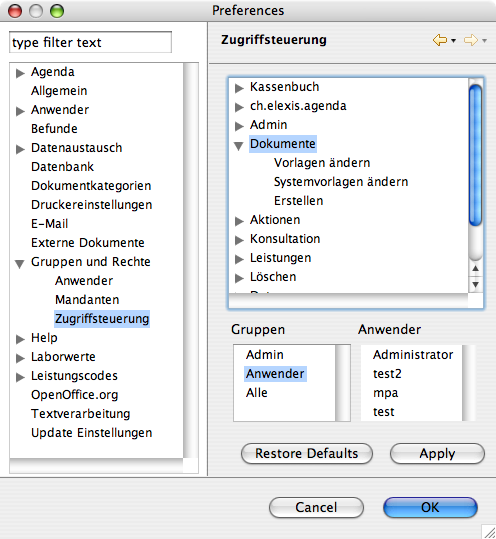
\includegraphics{images/zugriff}
  \caption{Zugriffssteuerung}
  \label{fig:zugriff}
\end{center}
\end{figure}

Comme vous pouvez constater les droits sont mentionnés et classés de manière hiérarchique.  -
Le droit \glqq changer modèle\grqq{} est évidemment subordonné au droit \glqq
documents\grqq{}. Dans la partie inférieure de la fenêtre vous trouvez tous les groupes et utilisateurs du système. 
Les règles du 'jeu' :
\begin{itemize}
  \item Avoir un droit implique aussi tout les droits qui lui sont subordonnées.
  \item Avoir un droit n'implique \textit{pas} automatiquement les droits maître.
  \item Chacun a les droits des rôles auxquels ils est inscrit et en sus ceux qui lui ont été attribués individuellement.
  \item Celui auquel on a attribué le rôle \glqq Admin\grqq a tout les droits même s'ils ne lui sont pas attribués de façon explicite.
  \item Celui à qui on a attribué \glqq les droits d'accès \grqq peut lui-même administrer les droits d'accès même s'il n'est pas administrateur.
\end{itemize}

On peut donc attribuer des droits d'accès à des rôles (groupes) ou individuellement aux utilisateurs. On attribue les droits de façon suivante : Cliquez avec la touche gauche dans la partie supérieure de la fenêtre sur le droit à attribuer et ensuite vous choisissez dans le champ inférieur un rôle ou un utilisateur en cliquant avec la touche gauche ou avec  [STRG]+ touche gauche s'il s'agit de plusieurs.

\textbf{Important:}N'oubliez pas la règle fondamentale : Personne, même pas le Chef, ne doit travailler sous le login 'admin' ou avoir que le rôle 'admin'. Le risque est trop grand de juste faire une 'petite' faute qui efface des données importantes. Si vous êtes le patron installez pour vous même deux différents 'accounts'.:
\begin{itemize}
  \item Un utilisateur simple (par ex. Dr Test) qui a le rôle d'un utilisateur ou d'un médecin et qui aura juste les droit d'accès dont il a besoin pour le travail journalier, mais surtout pas celui de 'l'admin'.
  \item Un administrateur (par ex. admin du cabinet) qui a le rôle d'admin et dont le mot de passe est strictement réservé à vous, même si vous avez toute confiance en votre personnel. Ne faites un login sur cet account que si vous devez faire exceptionnellement des choses qui ne sont pas faisable depuis un autre account.
\end{itemize}

\section{Définition du profil des utilisateurs}
Dans un petit cabinet on apprécie souvent la capacité de Elexis d'aménager le poste de travail de façon très individuelle. L'assistante médicale peut arranger son écran avec d'autres layouts ou d'autres couleurs que le médecin. Dans un cabinet plus grand où les usagers doivent parfois changer leurs postes de travail, une certaine 'unité de doctrine' pour tous ou au moins pour toutes les personnes avec le même rôle est souhaitée. Elexis permet pour cela une configuration des couleurs et layouts.

\subsection{Réglages individuelles du programme}
Sous \textsc{fichier - options - utilisateur} vous pouvez définir la couleur et le design, des raccourcis de clavier, et le type de la barre de lancement rapide. Vous pouvez sauvegarder ces réglages sous un nom quelconque, introduisez pour cela un nom et cliquez sur \glqq sauvegarder réglage sous\grqq{}.

Depuis un autre poste de travail et sous un autre login vous pouvez faire les mêmes changements plus facilement en chargeant les mêmes réglages. Introduisez pour cela le nom et cliquez sur \glqq charger le réglage de\ldots\grqq{}.

\subsection{Mise en page individuelle des perspectives}
La disposition des fenêtres, donc la perspective, avec laquelle vous travaillez normalement, peut être adaptée individuellement. Ce réglage est lié au poste de travail (puisqu'il est aussi dépendant de l'écran installé). Vous pouvez aussi sauvegarder certaines aménagements de perspectives sous un nom spécifique pour pouvoir les réinstaller sur un autre poste. Introduisez pour la sauvegarde le nom spécifique et cliquez sur \glqq
sauvegarder l'aménagement du poste sous\ldots\grqq{}.

Pour copier ce réglage sur un autre poste de travail ouvrez : \textsc{fichier - options - utilisateur} et introduisez le nom en question pour cliquer ensuite sur \glqq charger le réglage du poste de travail de\grqq{}.


